\documentclass{hw-template}
\date{\today}
\author{Kyle Hansen}
\title{NE 523 HW4}

\newcommand{\p}{\ensuremath{^{\prime}}}

\usepackage{cancel}

\begin{document}
\maketitle

\section{Laplacian Adjoint}


The adjoint of $\mathbf{L}$ is defined using

\begin{equation}
    \left(g, \mathbf{L}f\right) = \left(f, \mathbf{L}^\dagger g\right).
\end{equation}

Expanding the inner product, the LHS becomes

\begin{equation}
    \left(g, \frac{\partial^2 f}{\partial x^2}\right) = \int_{-a}^{a}\; g(x)f^{\prime\prime}(x)dx.
\end{equation}

Applying integration by parts,

\begin{equation}
    \left(g, \frac{\partial^2 f}{\partial x^2}\right) = \left[ g(x) f\p(x)\Big|_{-a}^a -     \int_{-a}^{a}\; g\p(x)f\p(x)dx   \right],
\end{equation}

and expanding once more,

\begin{equation}
    \left(g, \frac{\partial^2 f}{\partial x^2}\right) = \left[ g(x) f\p(x)\Big|_{-a}^a -     \cancel{g\p(x)f(x)\Big|_{-a}^a} + \int_{-a}^{a}\; f(x) g^{\prime\prime}(x) dx  \right],
\end{equation}

where the second term becomes zero since $f(-a) = f(a) = 0$. Further using the fact that $f\p(-a) = -f\p(a)$, this becomes

\begin{equation}
    \left(g, \frac{\partial^2 f}{\partial x^2}\right) = \left[ f\p(a)\left(g(a) + g(-a) \right) + \int_{-a}^{a}\; f(x) g^{\prime\prime}(x) dx  \right]
\end{equation}

Then, \textit{if} $g(-a) = g(a) =0$, 

\begin{equation}
    \left(g, \frac{\partial^2 f}{\partial x^2}\right) = \left(f, \frac{\partial^2 g}{\partial x^2}\right)
\end{equation}

and thus the operator $\mathbf{L}$ is self-adjoint.

\section{Orthogonality of Laplacian Eigenfunctions}

\subsection{}

The solution takes the form

\begin{equation}
    f(x) = b\cos(\lambda x) + d\sin(\lambda x),
\end{equation}

and since the solution must be symmtric, $d = 0$ and thus

\begin{equation}
    f(x) = b\cos(\lambda x).
\end{equation}

For the boundary conditions to be satisfied, $\lambda a$ must be an odd-integer multiple of $\pi/2$ and thus the positive eigenvalues are

\begin{equation}
    \lambda_n = \frac{(2n+1)\pi}{2a}.
\end{equation}

where $n=0, 1, \dots$. The associated eigenfunctions are

\begin{equation}
    f_n(x) = \cos \left(\frac{(2n+1)\pi}{2a} x \right)
\end{equation}

To simplify notation, let $m$ and $\ell$ be positive odd integers. Then the inner product of two eigenfunctions is

\begin{equation}\label{eq:og-integral}
    \int_{-a}^a \cos \left(\frac{\pi m x}{2a} \right)\cos\left(\frac{\pi \ell x}{2a} \right)dx
\end{equation}

which can be expressed

\begin{equation}
    \frac{1}{2}\int_{-a}^a \cos \left(\frac{\pi (m+\ell) x}{2a} \right) + \cos\left(\frac{\pi (m - \ell) x}{2a} \right)dx
\end{equation}

which is equal to 

\begin{equation}
    \frac{1}{2} \left[ \frac{2}{\pi (m + \ell)}\sin\left(\frac{\pi (m+\ell) x}{2a} \right) + \frac{2}{\pi (m - \ell)} \cos \left(\frac{\pi (m - \ell) x}{2a} \right) \right]_{-a}^a.
\end{equation}

Since $m+\ell$ and $m-\ell$ are both even integers, the terms inside the sine become integer multiples of $\pi$ at the bounds, and thus the inner product is zero if $m\neq \ell$.

\subsection{}

Since $\varphi$ can be represented using a linear combination of the eigenfunctions,

\begin{equation}
    -\frac{d^2\varphi}{dx^2} = -\sum_{n=0}^{\infty}\alpha_n \frac{d^2 f_n}{dx^2} = \sum_{n=0}^{\infty}\alpha_n \lambda_n^2 f_n(x) = S
\end{equation}

then the coefficients are found using orthogonality by multiplying by a particular eigenfunction and integrating over the domain,

\begin{equation}
    \int_{-a}^a \sum_{n=0}^{\infty}\alpha_n \lambda_n^2 f_n(x)f_m(x) dx = \alpha_m\lambda_m^2 \int_{-a}^a  f_m(x)^2 dx  = S\int_{-a}^a f_m(x)dx
\end{equation}

and thus 

\begin{equation}
    \alpha_m = \frac{S}{\lambda_m^2} \frac{\int_{-a}^a f_m(x)dx}{\int_{-a}^a  f_m(x)^2 dx}
\end{equation}

where the integral of $f$ finally evaluates to

\begin{equation}
    \int_{-a}^a f_m(x)dx = \int_{-a}^a \cos \left(\frac{(2+1)\pi}{2a} x \right) dx = (-1)^m\frac{4a}{(2m-1)\pi}
\end{equation}

and 

\begin{equation}
    \int_{-a}^a f_m(x)^2dx = a,
\end{equation}

so

\begin{equation}
    \alpha_m = (-1)^{m}\frac{S}{\lambda_m^2} \frac{4}{(2m+1)\pi}
\end{equation}

and the solution is 

\begin{equation}
    \varphi(x) = \sum_{n=1}^\infty \alpha_n f_n(x).
\end{equation}

\subsection{}

The analytical solution is

\begin{equation}
    \varphi(x) = \frac{S}{2}\left(a^2 - x^2 \right).
\end{equation}

The truncated consine reconstructions are shown in \autoref{fig:figures}, where $S=1$ and $a=1$.

\begin{figure}
    \centering
    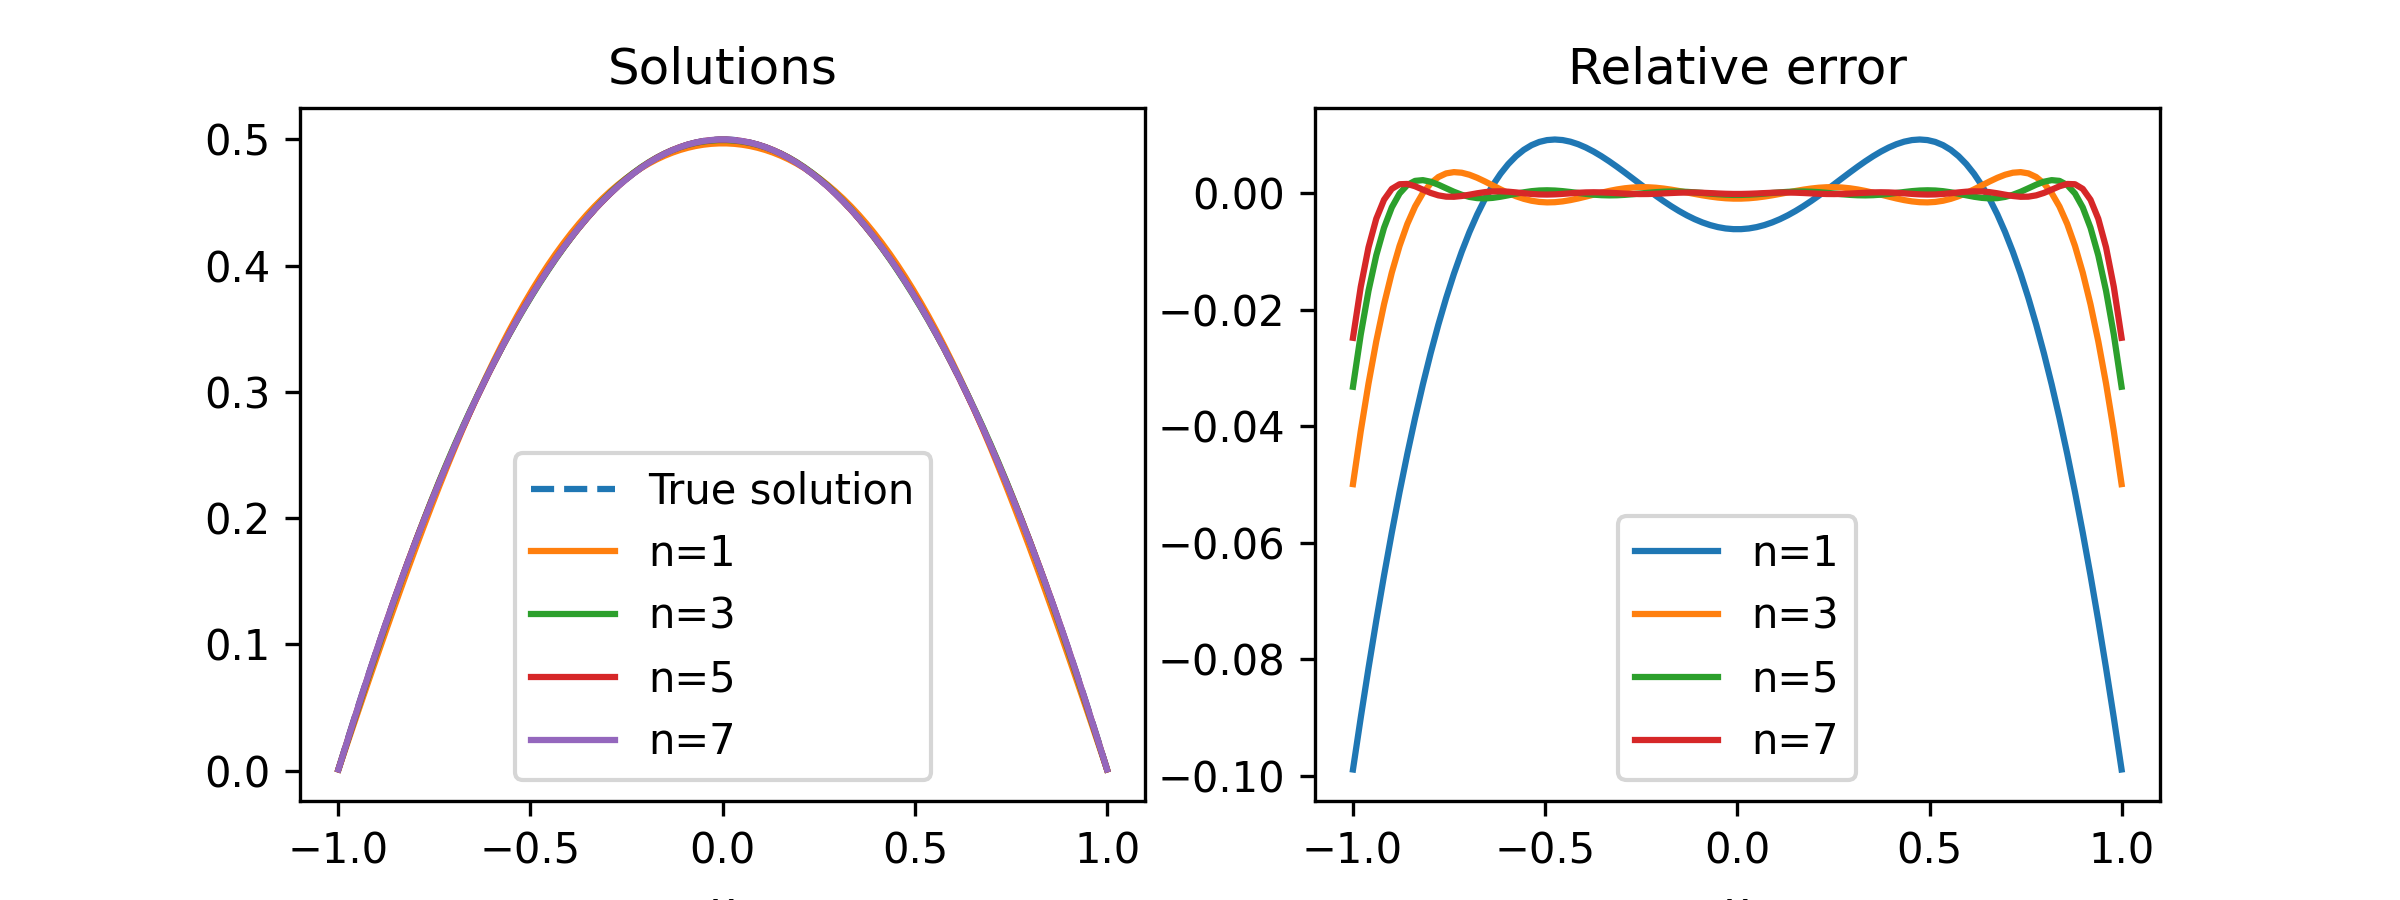
\includegraphics[width=\linewidth]{figure.png}
    \caption{Solutions and Errors}\label{fig:figures}
\end{figure}









\end{document}